
\subsection*{Partie A : Lecture graphique}

\paragraph{1.} La tangente en \(A\) est horizontale donc \(f'(0) = 0\).

La tangente en \(B\), qui est la droite \((BC)\), a pour coefficient directeur :
\[
f'(2) = \dfrac{6 - 2}{1 - 0} = 4.
\]

\subsection*{Partie B : Calcul algébrique}

\(f(x) = \e^x (2x + 2)\).

\paragraph{2.} En tant que produit de fonctions dérivables sur \(\mathbb{R}\), \(f\) est dérivable sur \(\mathbb{R}\) et :
\[
f'(x) = \e^x (2x + 2) + 2\e^x = \e^x(2x + 2 + 2) = \e^x(2x + 4).
\]

\paragraph{3.} On sait que, quel que soit le réel \(x\), \(\e^x > 0\), donc le signe de \(f'(x)\) est celui de \(2x + 4\).

\[
2x + 4 > 0 \iff x > -2
\]

Donc \(f\) est décroissante sur \(\left]-\infty\,;\,-2\right[\), puis croissante sur \(\left]-2\,;\,+\infty\right[\), avec un minimum en :
\[
f(-2) = \e^{-2}(2 \times (-2) + 2) = -2 \e^{-2} \approx -0{,}271.
\]

\begin{center}
\begin{tikzpicture}
\tkzTabInit[lgt=3, espcl=3]{$x$ / 1, {$\e^x$} / 1, {$2x + 4$} / 1, {Signe de $f'(x)$} / 1, {$f$} / 2}{${-\infty}$, ${-2}$, ${+\infty}$}
\tkzTabLine{,+,,+,}
\tkzTabLine{,-,0,+,}
\tkzTabLine{,-,0,+,}
\tkzTabVar{+/{$$},-/{$-2\e^{-2} \approx -0{,}271$},+/{$$}}{/}
\end{tikzpicture}
\end{center}

\paragraph{4.} On sait que l'équation réduite de la tangente au point d'abscisse \(0\) est :
\[
y - f(0) = f'(0)(x - 0).
\]
Avec \(f(0) = 1 \times 2 = 2\) et \(f'(0) = 1 \times (0 + 4) = 4\), l'équation devient :
\[
y - 2 = 4x \quad \text{ou} \quad y = 4x + 2.
\]

\paragraph{5.}
La tangente en \(A\) est parallèle à l'axe des abscisses.  
\(A\) a pour abscisse \(-2\), donc :
\[
f'(-2) = \e^{-2} \times (2 \times (-2) + 4) = \e^{-2} \times 0 = 0,
\]
la tangente en \(A\) est parallèle à l'axe des abscisses.

L'équation de la tangente étant \(y = 4x + 2\), on a bien pour \(x = 1\) (abscisse de C) :
\[
y = 4 \times 1 + 2 = 6 \text{ (ordonnée de C).}
\]
La tangente en \(B\) contient bien le point \(C\).

